% !TeX root = ../thesis.tex

%%%%%%%%%%%%%%%%%%%%%%%%%%%%%%%%%%%%%%%%%%%%%%%%%%%%%%%%%%%%%%%%%%% 
%                                                                 %
%                            CHAPTER                              %
%                                                                 %
%%%%%%%%%%%%%%%%%%%%%%%%%%%%%%%%%%%%%%%%%%%%%%%%%%%%%%%%%%%%%%%%%%% 
 
\chapter{Design and validation}

The design of a single-stage transmitter is built around a Pierce oscillator (shown in Figure~\ref{fig:pierce_main}); this is a circuit built out of a crystal, two capacitors, and an inverter. It works by inducing a $180^\circ$ phase shift through the crystal and capacitor network and then inverting and amplifying that signal. This circuit has a total $360^\circ$ phase shift and an amplification greater than 1, fulfilling the Barkhausen criterion. The single-stage transmitter makes use of a crystal, and the two capacitors come from the base-emitter capacitance of the transistor and the capacitively tuned LC tank network. The transistor acts as an inverter/amplifier. The base resistor regulates the bias current, and the base RC network makes the oscillator pulse. A detailed explanation of the oscillator circuit can be found in Appendix~\ref{app:crystal}.

\begin{figure}[htbp]
	\centering
	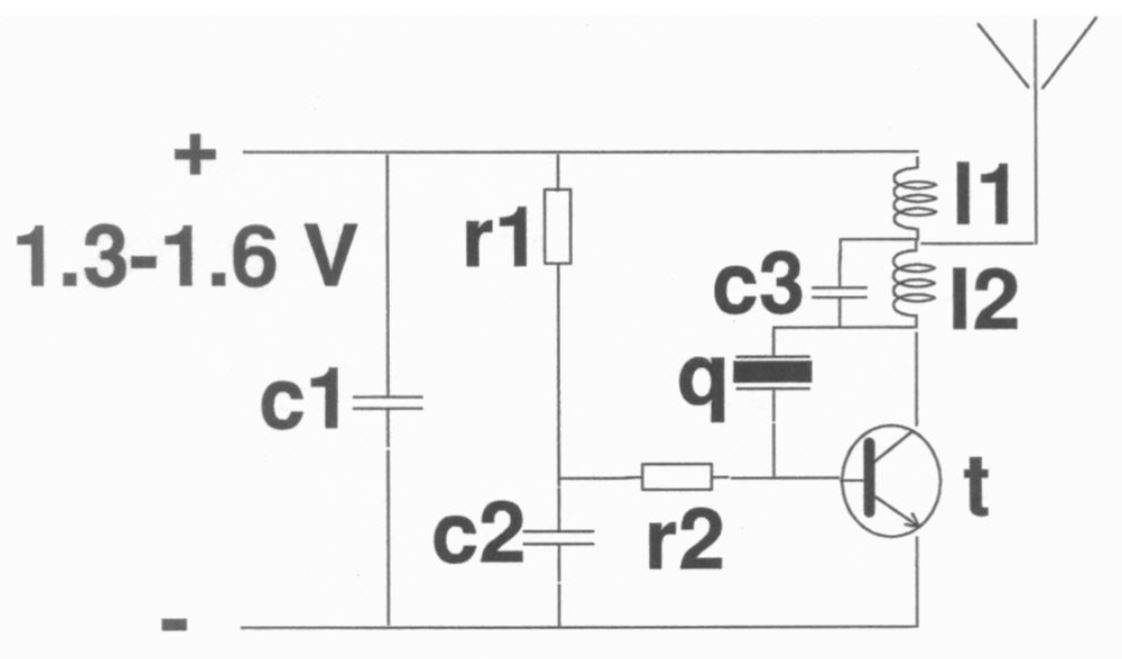
\includegraphics[width=0.5\textwidth]{Single_Stage_Transmitter_Circuit.JPG}
	\caption{Schematic of the single-stage Pierce oscillator circuit (taken from \cite{naef-daenzerNewTransmitterSmall1993a}).}
	\label{fig:pierce_main}
\end{figure}
 
\section{Component calculation}

\section{Simulation}
 
\section{prototype testing}